\documentclass{beamer}


\graphicspath{ {images/} }

\usetheme{Boadilla}

\title{Spotting Distracted Drivers}
\subtitle{HLCV Project}
\author[Reyes, Schaefer, Tonsen, Weber]{Guillermo Reyes \\
	 Daniel Schaefer \\
	 Marc Tonsen \\
 Dominik Weber\\}
 \institute[]{Saarland University}
\date{20.06.2016}



\begin{document}
	\begin{frame}
		\titlepage
	\end{frame}
	
	
	\section{Tested but not working}	
	
	\begin{frame}
		\frametitle{Face Detection}
		Using all kinds of cascadeClassifier available in openCV. The results have been unsatisfactory so far mainly because our camera/face angle is very different, and even the profile detections don't work very well on pictures which come fairly close to being a profile view. Also a Problem would be occlusion, sun glasses and long hair. 
		different haar-cascades for example face-boxer.

		However some have had reasonable results
		\begin{itemize}
		\item Face detection, pose estimation and landmark localization in the wild
		\item Dlib (in part)  
		\end{itemize}
	\end{frame}
	
	\begin{frame}
		\frametitle{Correct Face detection}
		\begin{center}
			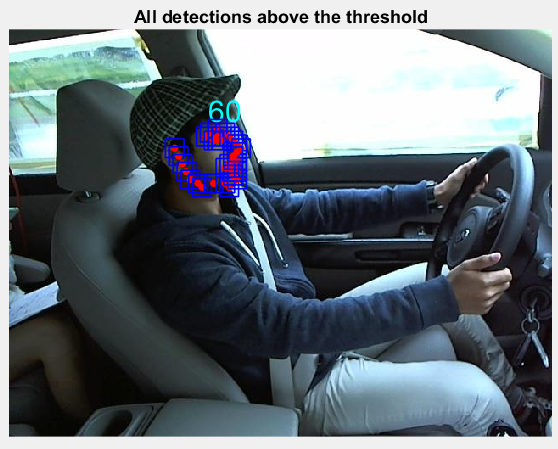
\includegraphics[width=0.4\textwidth]{faces/face1} \\ \vspace{0.1cm}
			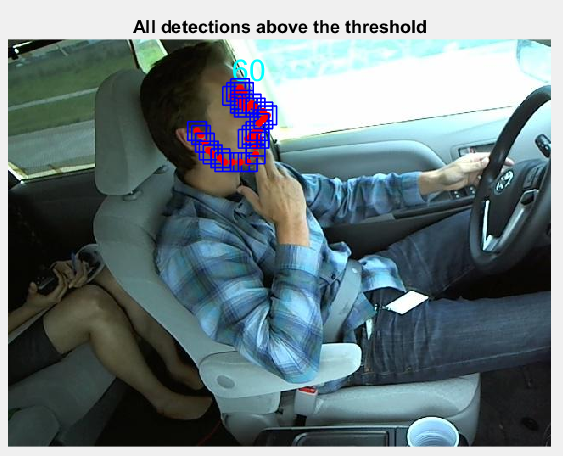
\includegraphics[width=0.35\textwidth]{faces/face4} \hspace{0.1cm}
			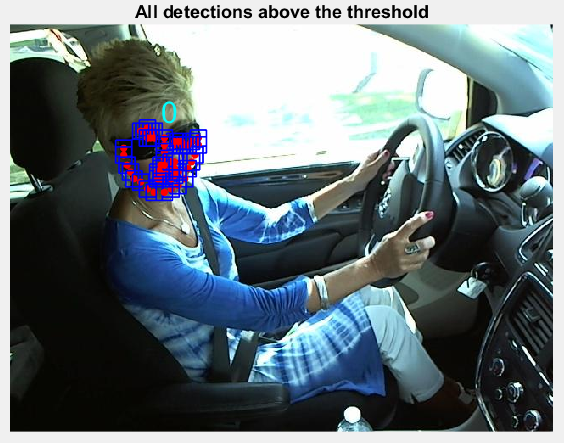
\includegraphics[width=0.35\textwidth]{faces/face6}
		\end{center}		
	\end{frame}
	\begin{frame}
		\frametitle{Incorrect Face detection}
		\begin{center}
			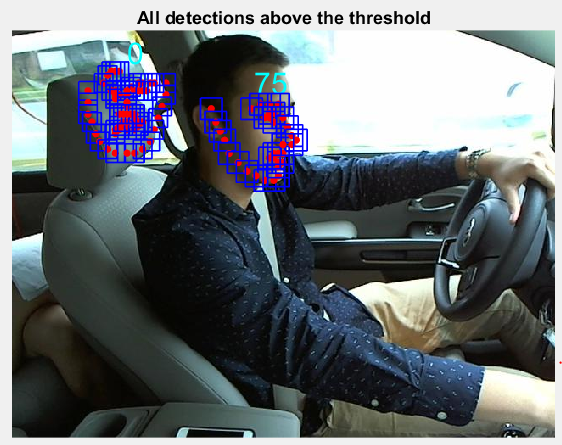
\includegraphics[width=0.4\textwidth]{faces/face3} \\ \vspace{0.1cm}
			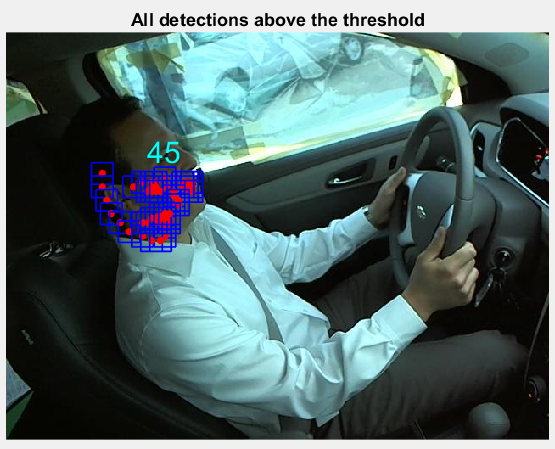
\includegraphics[width=0.35\textwidth]{faces/face5} \hspace{0.1cm}
			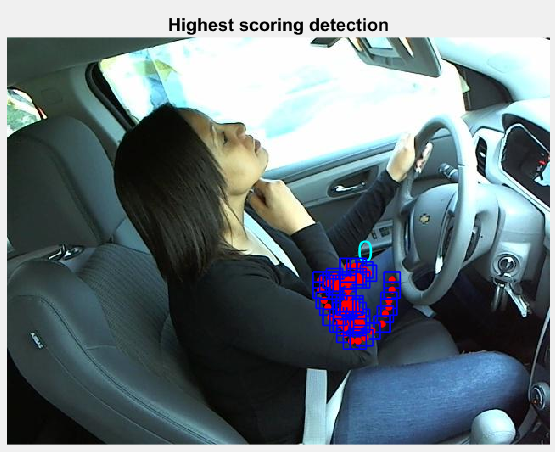
\includegraphics[width=0.35\textwidth]{faces/face7}
		\end{center}		
	\end{frame}
	
	\begin{frame}
		\frametitle{Dlib Face detection}
		\begin{center}
			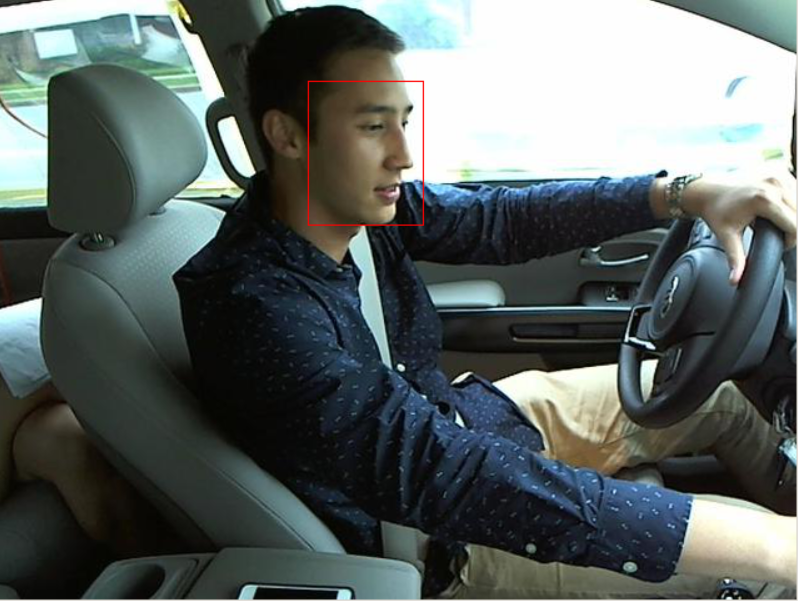
\includegraphics[width=0.4\textwidth]{faces/dlibface1} \\ \vspace{0.1cm}
			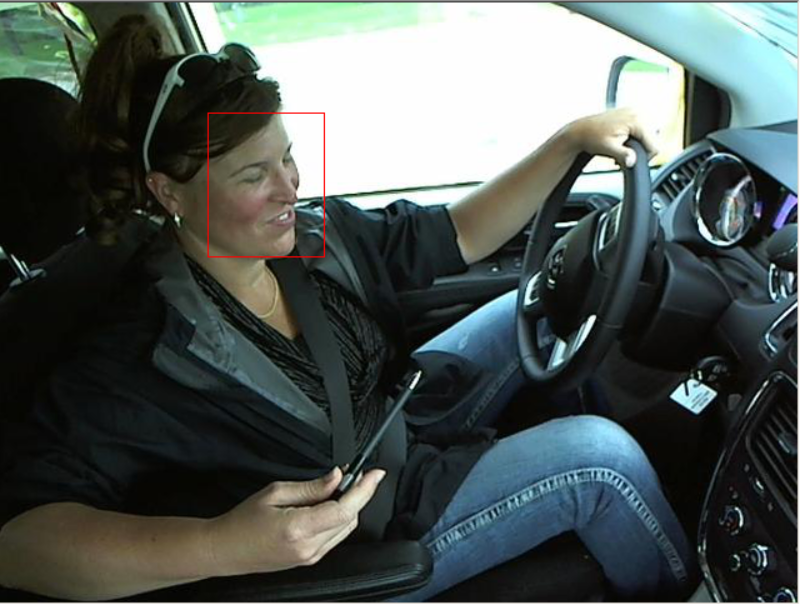
\includegraphics[width=0.35\textwidth]{faces/dlibface2} \hspace{0.1cm}
			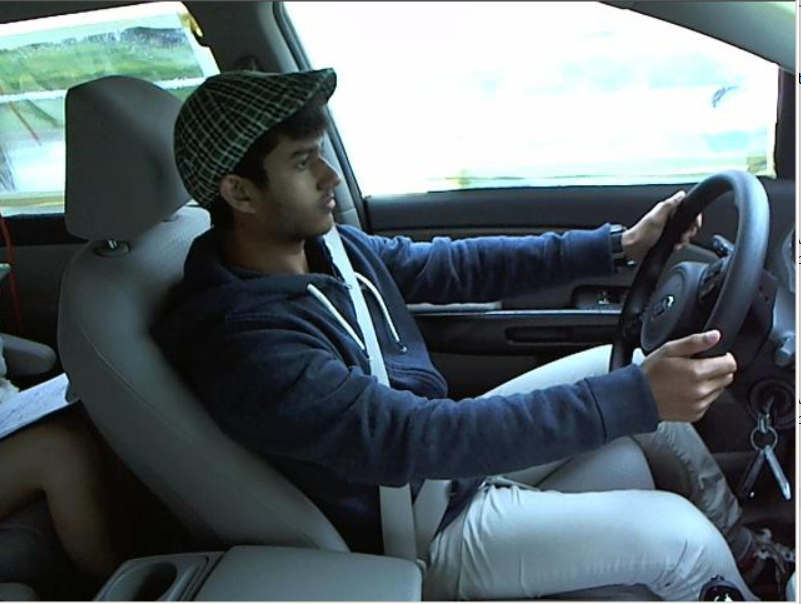
\includegraphics[width=0.35\textwidth]{faces/dlibface3}
		\end{center}		
	\end{frame}
    

	
	
\end{document}
